\documentclass{standalone}
\usepackage[T1]{fontenc}
\usepackage[utf8]{inputenc}
\usepackage[english]{babel}
\usepackage{tikz}
\usepackage{times}
\usepackage{tabularht}
\usetikzlibrary{calc,through,backgrounds,positioning,fit}
\usetikzlibrary{shapes,arrows,shadows}

\begin{document}

\begin{tikzpicture}



\node (tabela) [label = \textit{Data with clusters assigned}] at (0,0)  {
                    \begin{tabular}{|c|c|c|c|c||c|}
			\hline
			$t$ & $a_1$ & $a_2$ & $\ldots$ & $a_k$ &c \\
			\hline\hline
			
			$t_1$ & $v_1^1$ & $v_2^1$ & $\ldots$ & $v_k^1$ & $c_1$ \\ \hline
			$t_2$ & $v_1^2$ & $v_2^2$ & $\ldots$ & $v_k^2$ & $c_2$ \\ \hline
			$\ldots$ & $\ldots$ & $\ldots$ & $\ldots$ & $\ldots$ & $\ldots$ \\ \hline
			$t_n$ & $v_1^n$ & $v_2^n$ & $\ldots$ & $v_k^n$ & $c_n$ \\ \hline
			$\ldots$ & $\ldots$ & $\ldots$ & $\ldots$ & $\ldots$ & $\ldots$ \\ \hline

		\end{tabular}
};

\node (graf)[label=\textit{State graph}] at (7.4,0){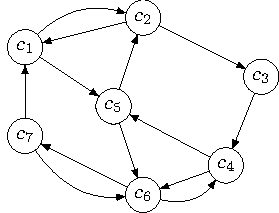
\includegraphics{statesgraph.pdf}};

\linespread{0.8};

\draw[->, gray, line width=3pt] (tabela) -- node [text width=2.5cm,above=-5pt,,align=center,black] {Process discovery} (graf) ;

\end{tikzpicture}
\end{document}